% Chapter Template

\chapter{Experimental Results} % Main chapter title

\label{Chapter4} % Change X to a consecutive number; for referencing this chapter elsewhere, use \ref{ChapterX}

\lhead{Chapter 4. \emph{Experimental Results}} % Change X to a consecutive number; this is for the header on each page - perhaps a shortened title

%----------------------------------------------------------------------------------------
%	SECTION 1
%----------------------------------------------------------------------------------------

\section{The Model}



%-----------------------------------
%	SUBSECTION 1
%-----------------------------------
\subsection{Small-World Networks}


%-----------------------------------
%	SUBSECTION 2
%-----------------------------------

\subsection{Scale-free Networks}


%----------------------------------------------------------------------------------------
%	SECTION 2
%----------------------------------------------------------------------------------------

\section{The Simulation}

%-----------------------------------
%	SUBSECTION 1
%-----------------------------------
\subsection{Color Histograms}


%-----------------------------------
%	SUBSECTION 2
%-----------------------------------

\subsection{Spatial Cluster}

%-----------------------------------
%	SUBSECTION 3
%-----------------------------------

\subsection{Cost-Gain Function}

\begin{figure}
\begin{center}$
\begin{array}{ccc}
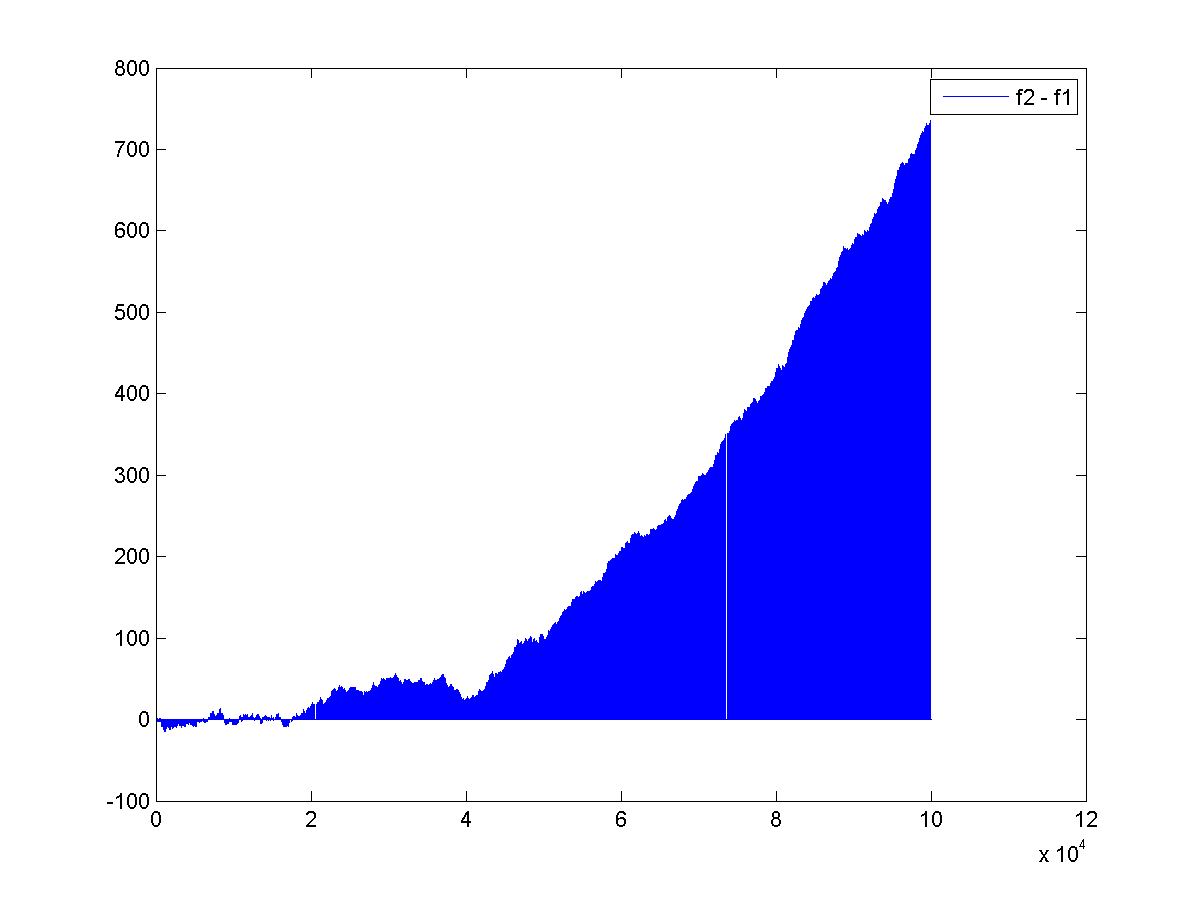
\includegraphics[scale=0.33]{Figures/base1/base1_1} 
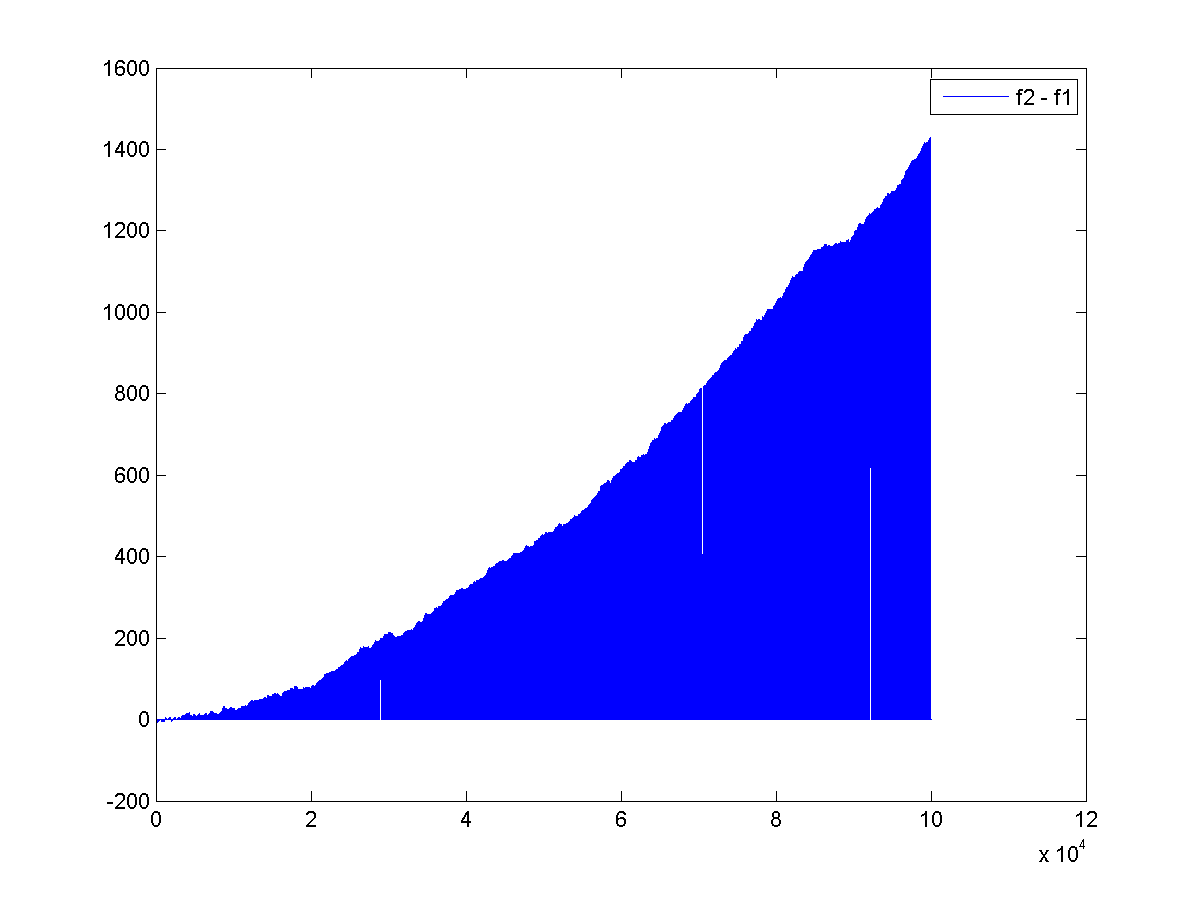
\includegraphics[scale=0.33]{Figures/base1/base1_2} \\
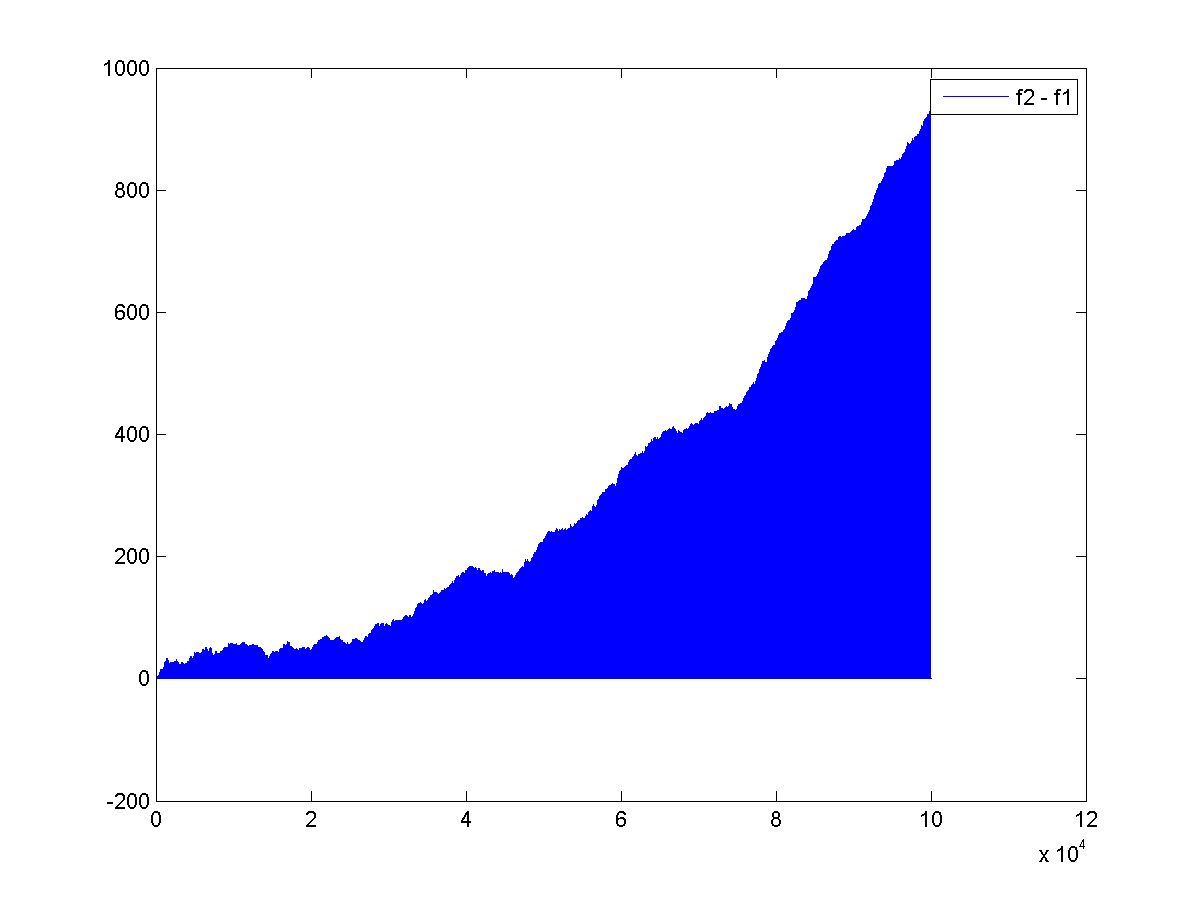
\includegraphics[scale=0.33]{Figures/base1/base1_3}
\end{array}$
\end{center}
\caption{Base 1}
\label{fig:base1}
\end{figure}

\begin{figure}
\begin{center}$
\begin{array}{ccc}
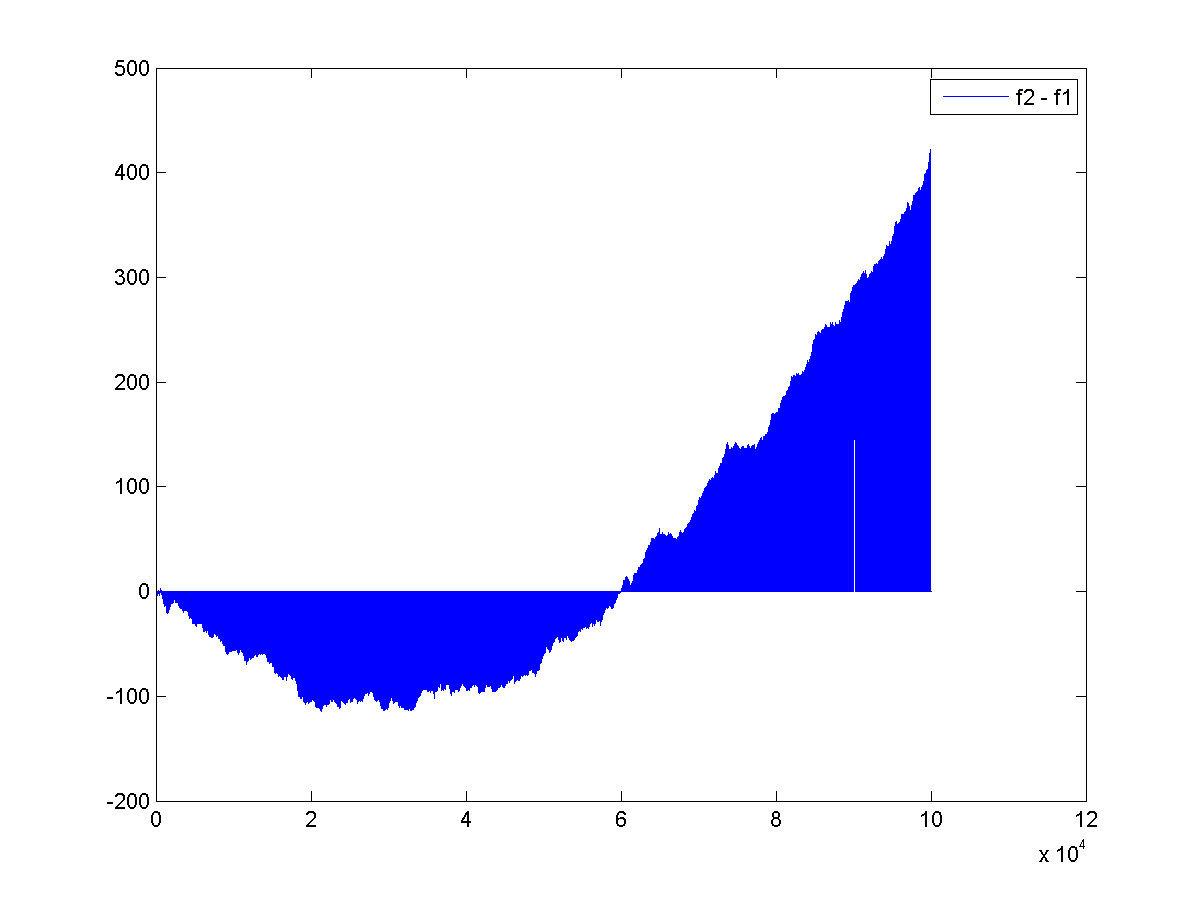
\includegraphics[scale=0.33]{Figures/base1/base2_1} 
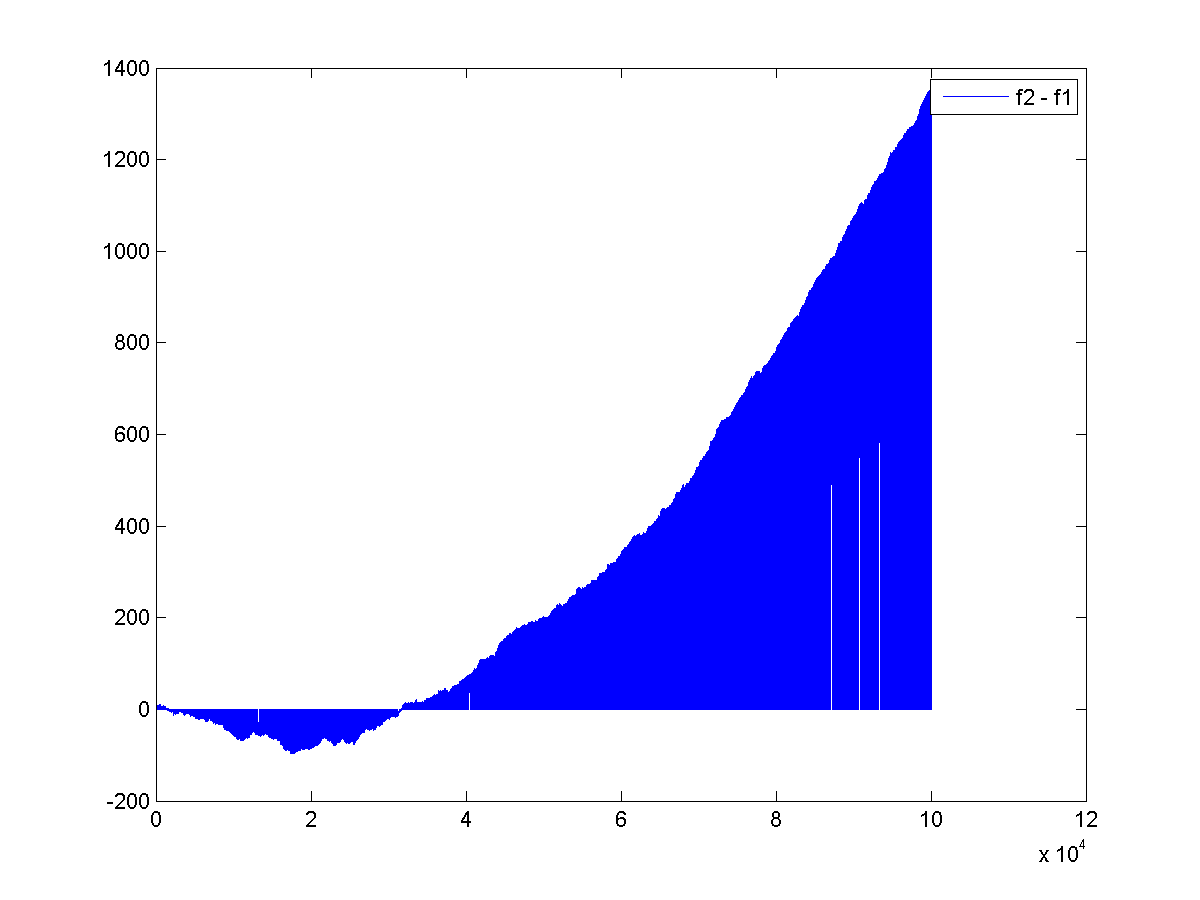
\includegraphics[scale=0.33]{Figures/base1/base2_2} \\
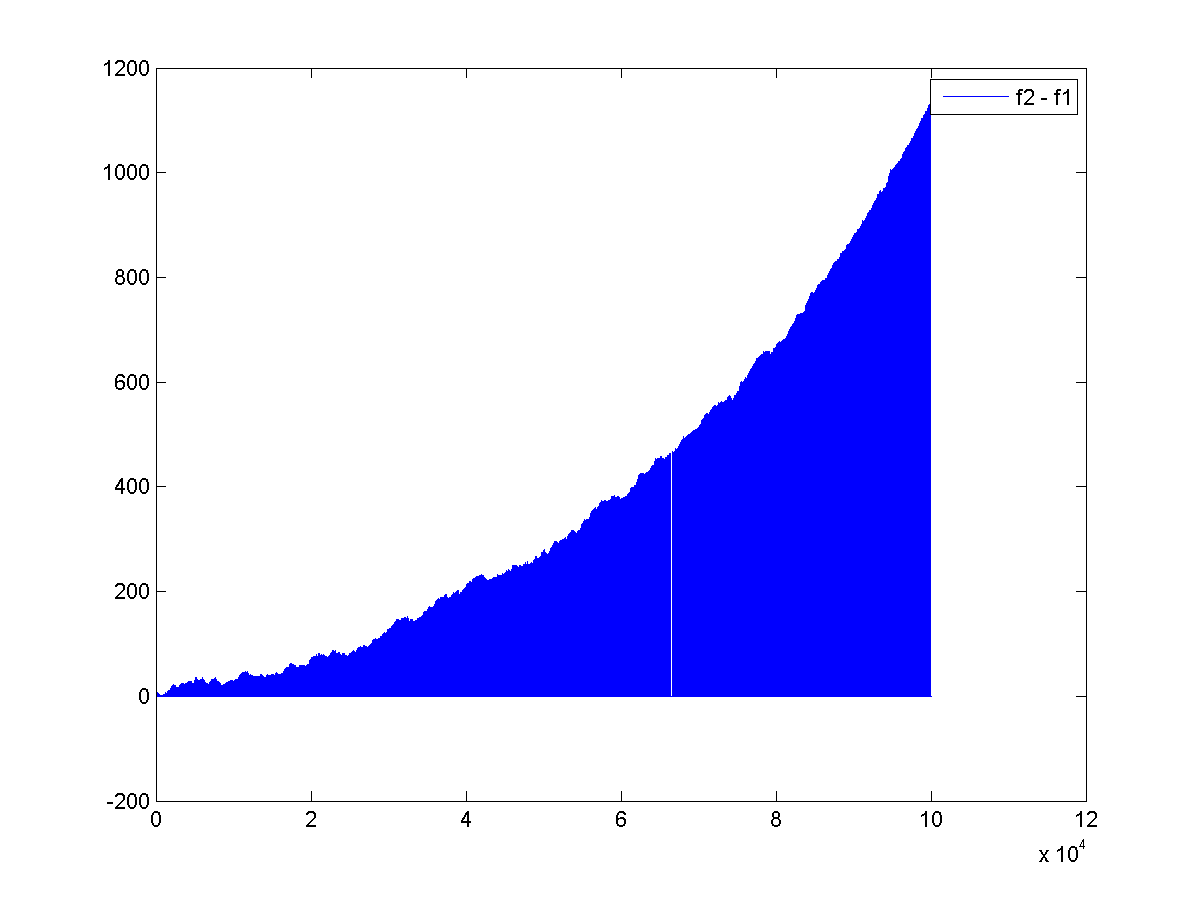
\includegraphics[scale=0.33]{Figures/base1/base2_3}
\end{array}$
\end{center}
\caption{Base 2}
\label{fig:base2}
\end{figure}

\begin{figure}
\begin{center}$
\begin{array}{ccc}
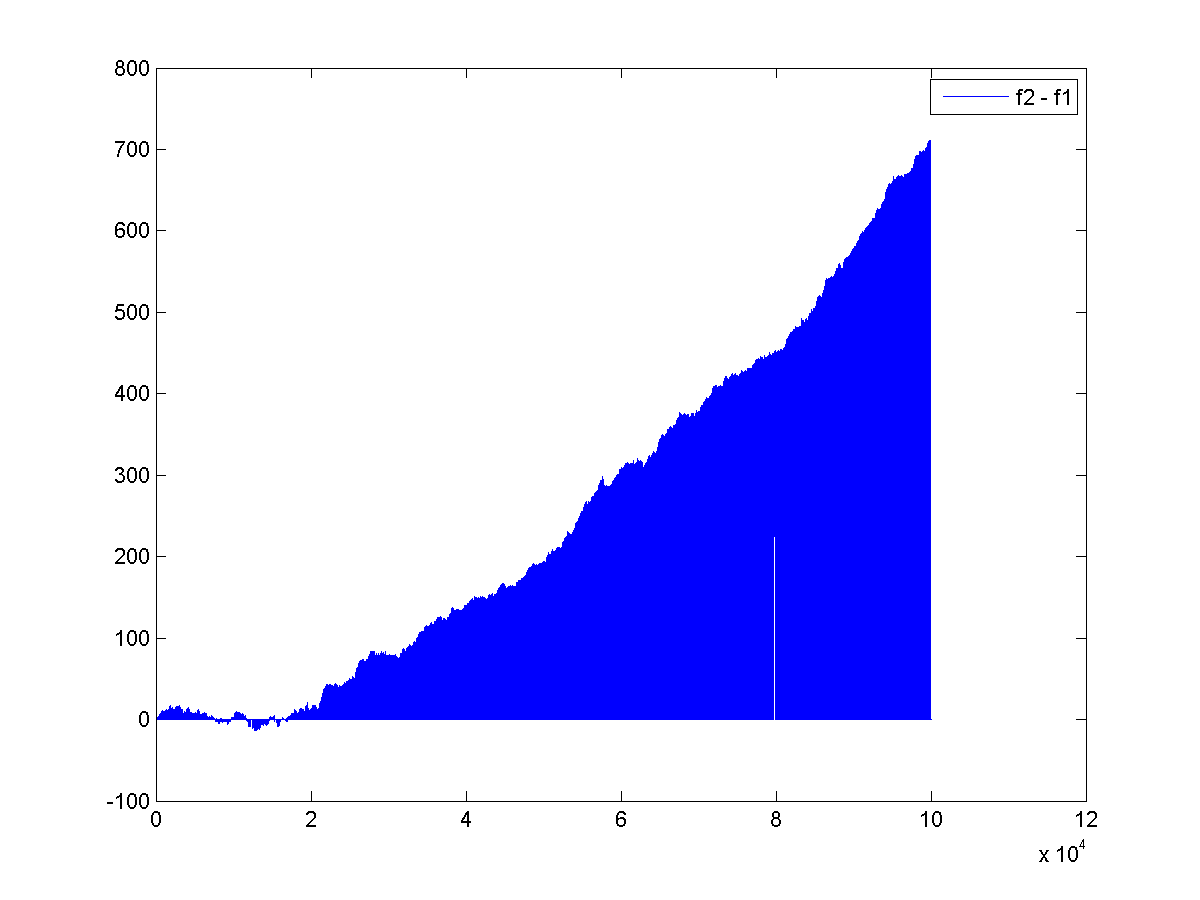
\includegraphics[scale=0.33]{Figures/base1/base3_1} 
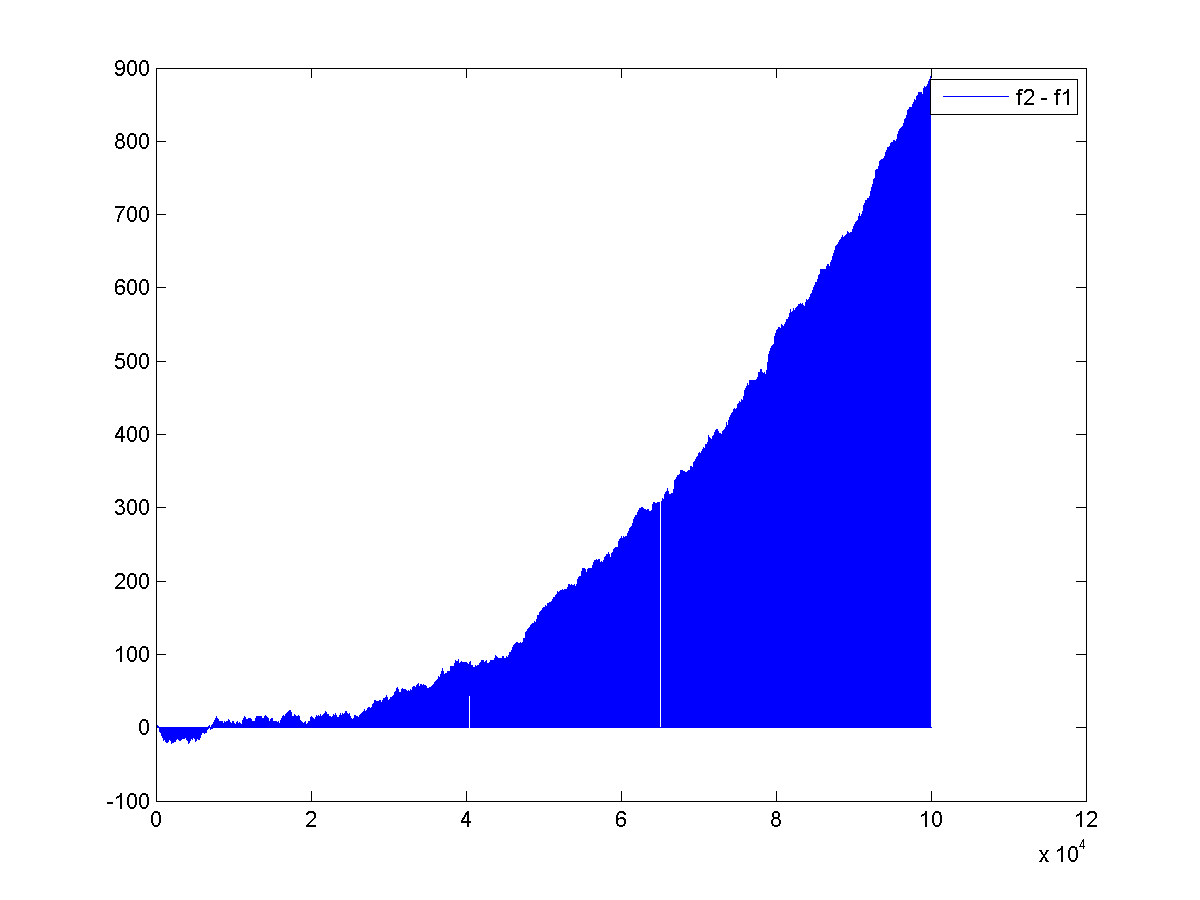
\includegraphics[scale=0.33]{Figures/base1/base3_2} \\
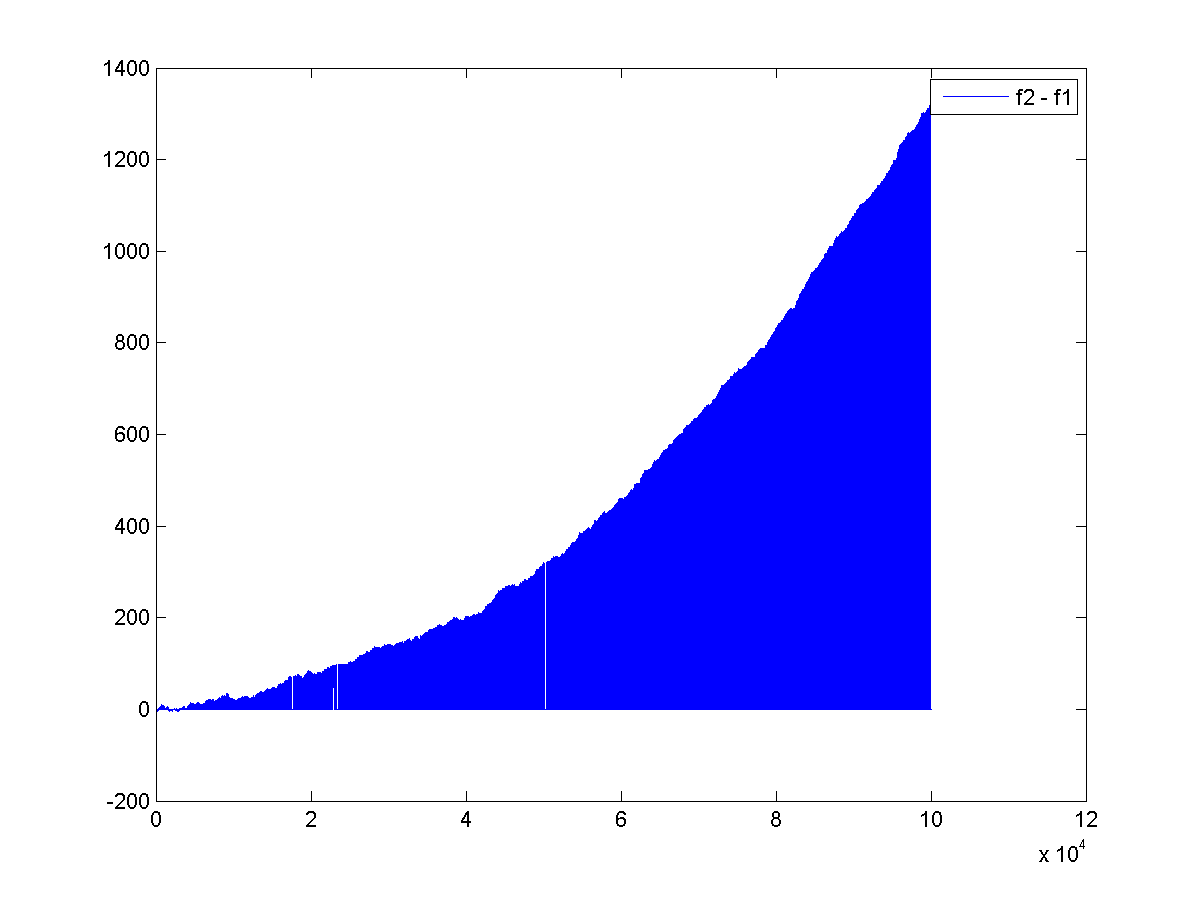
\includegraphics[scale=0.33]{Figures/base1/base3_3}
\end{array}$
\end{center}
\caption{Base 3}
\label{fig:base3}
\end{figure}

\begin{figure}
\begin{center}$
\begin{array}{ccc}
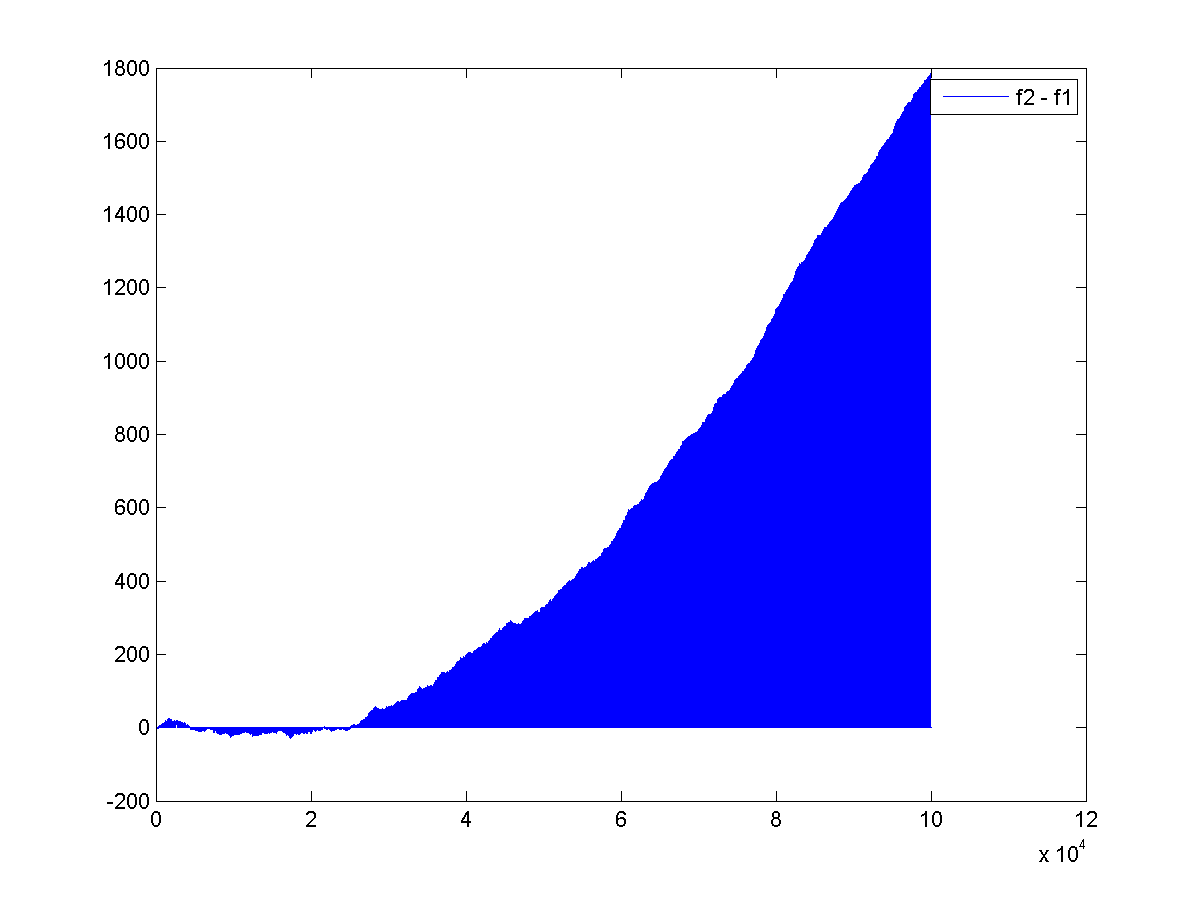
\includegraphics[scale=0.33]{Figures/base1/base4_1} 
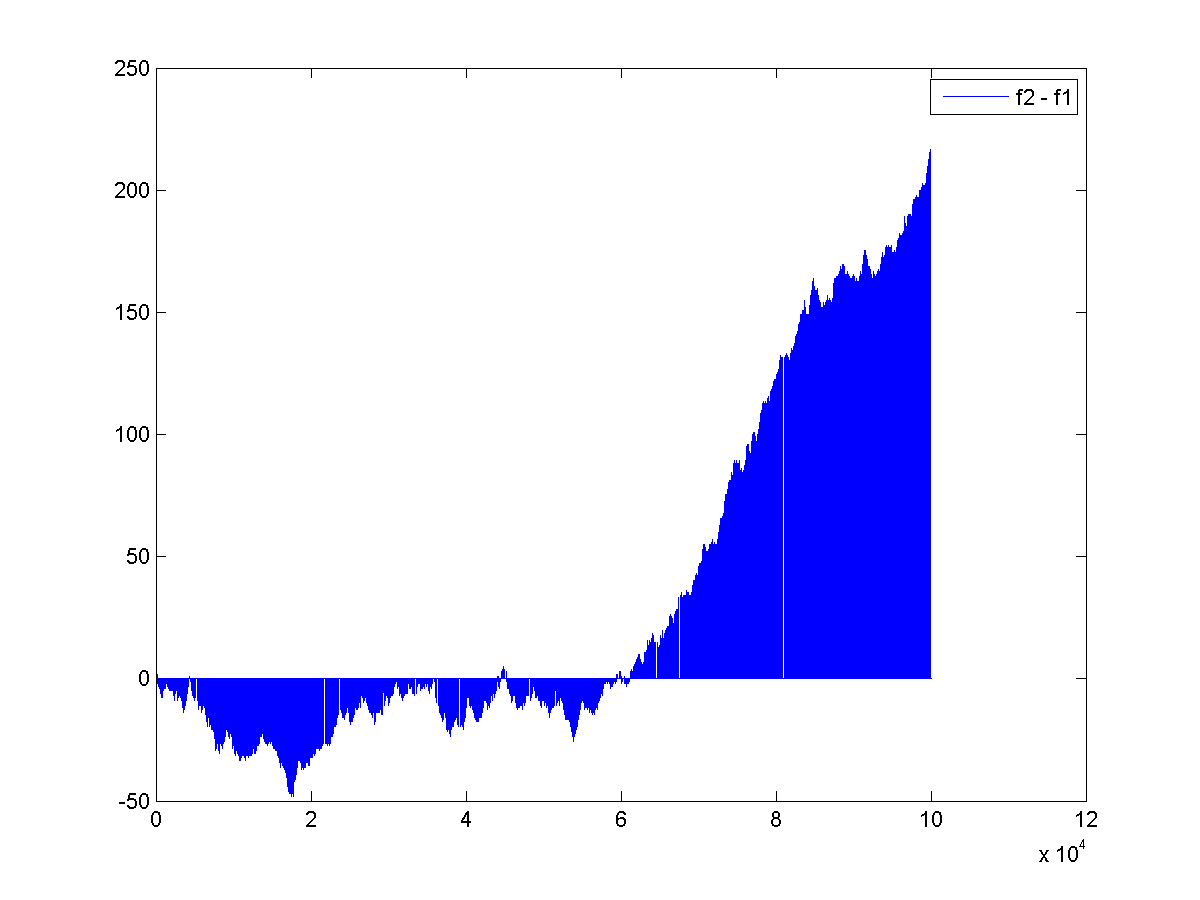
\includegraphics[scale=0.33]{Figures/base1/base4_2} \\
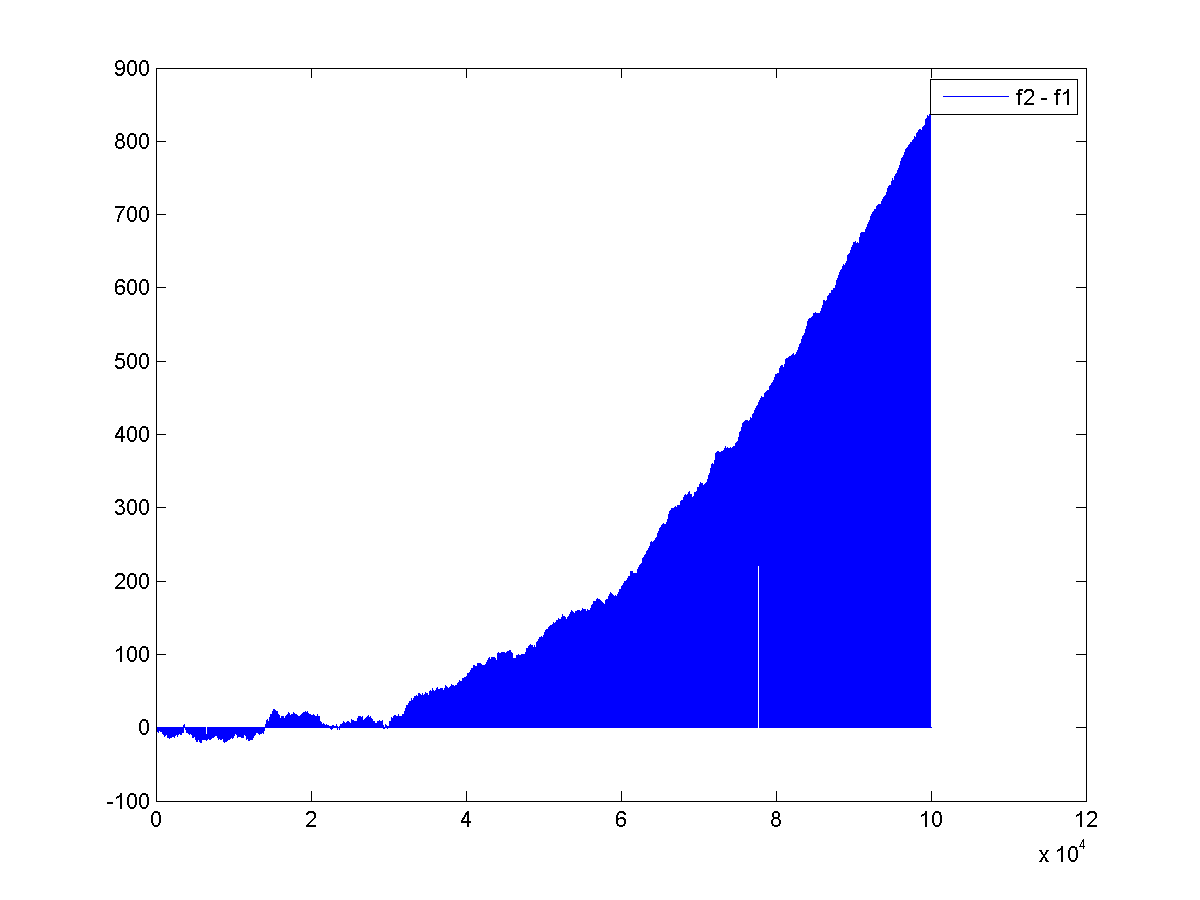
\includegraphics[scale=0.33]{Figures/base1/base4_3}
\end{array}$
\end{center}
\caption{Base 4}
\label{fig:base4}
\end{figure}

\begin{figure}
\begin{center}$
\begin{array}{ccc}
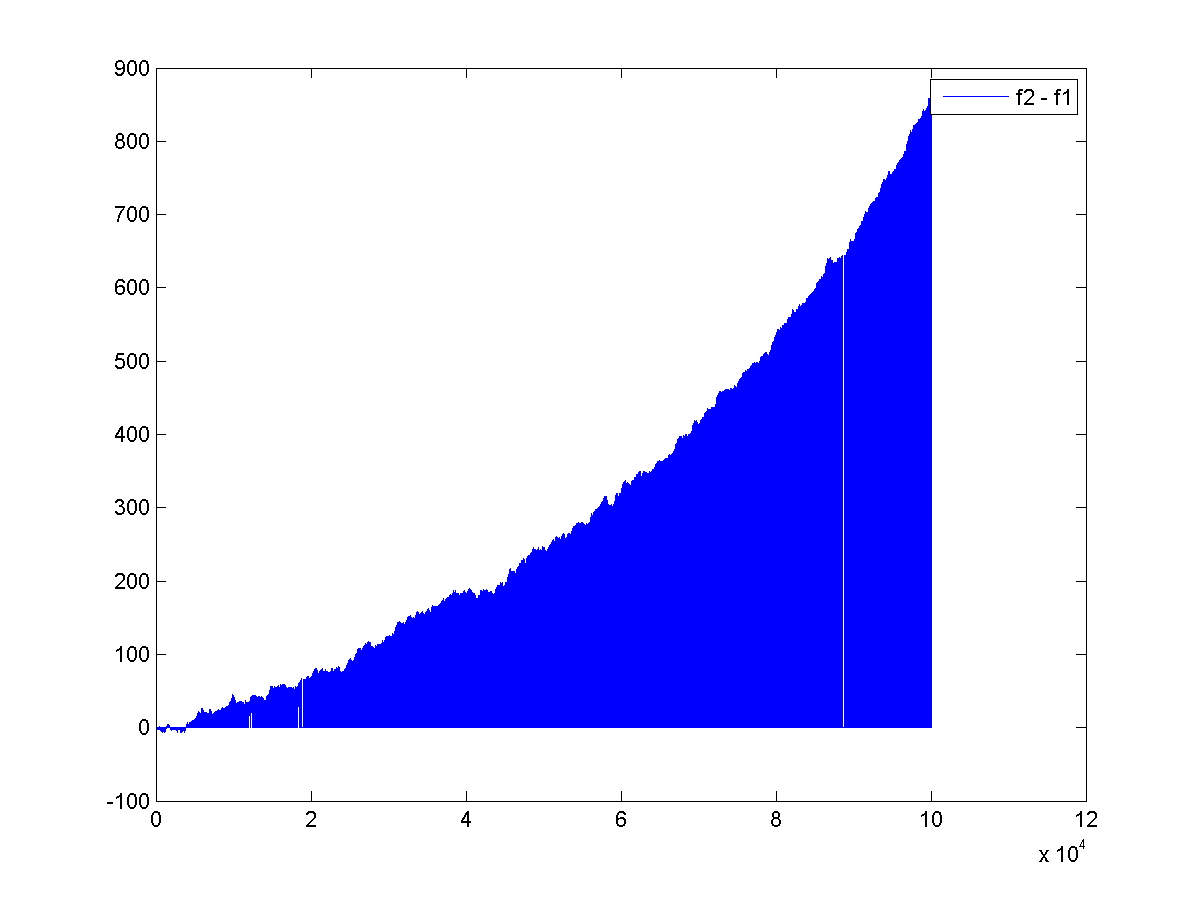
\includegraphics[scale=0.33]{Figures/base1/diff1_1} 
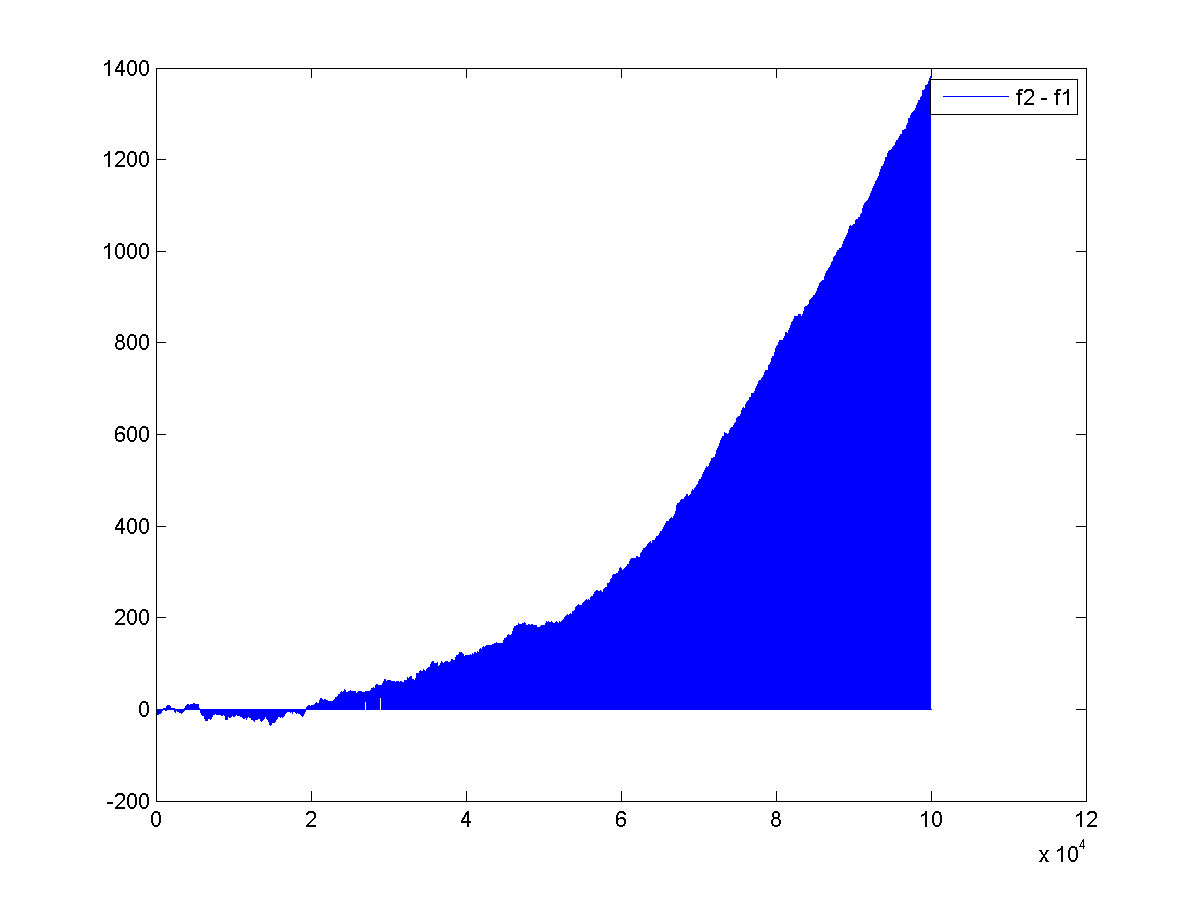
\includegraphics[scale=0.33]{Figures/base1/diff1_2} \\
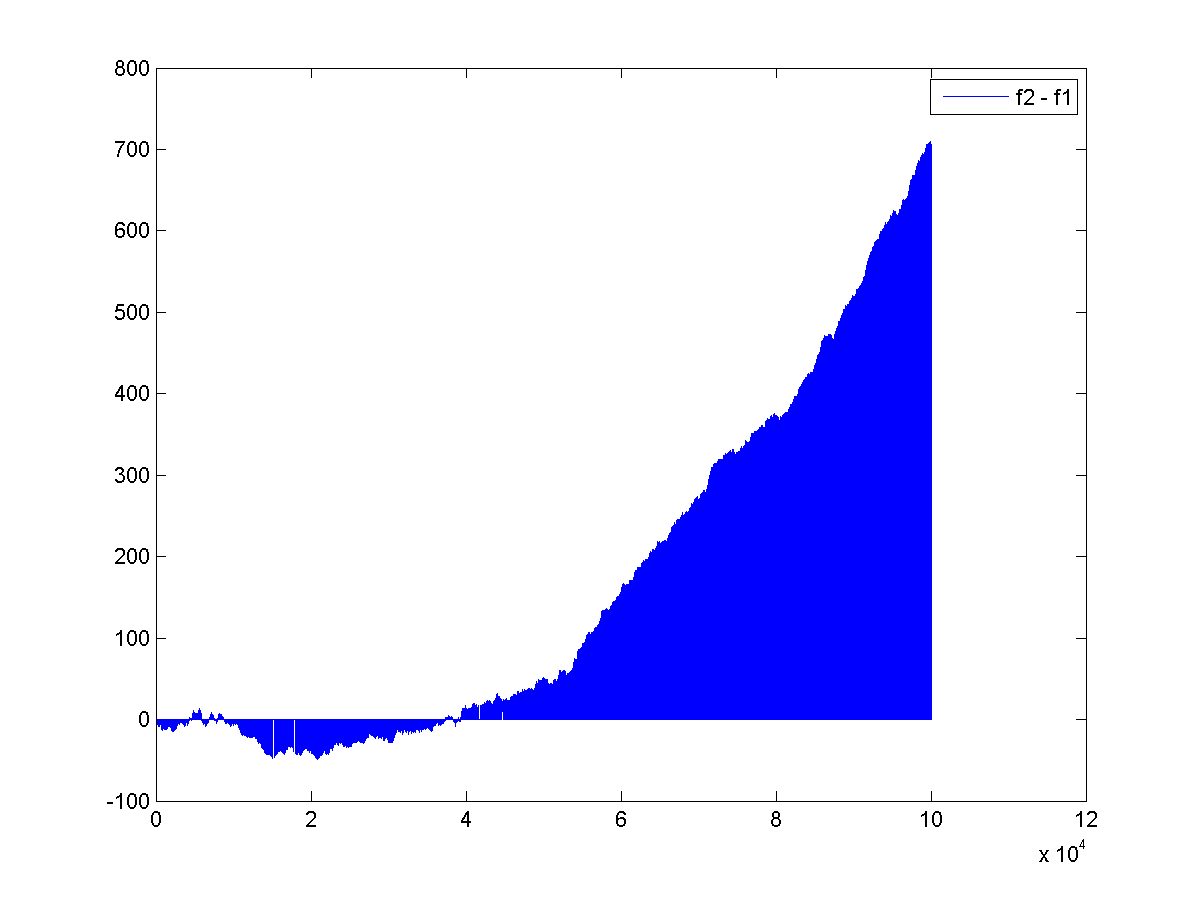
\includegraphics[scale=0.33]{Figures/base1/diff1_3}
\end{array}$
\end{center}
\caption{Difference 1}
\label{fig:diff1}
\end{figure}

\begin{figure}
\begin{center}$
\begin{array}{ccc}
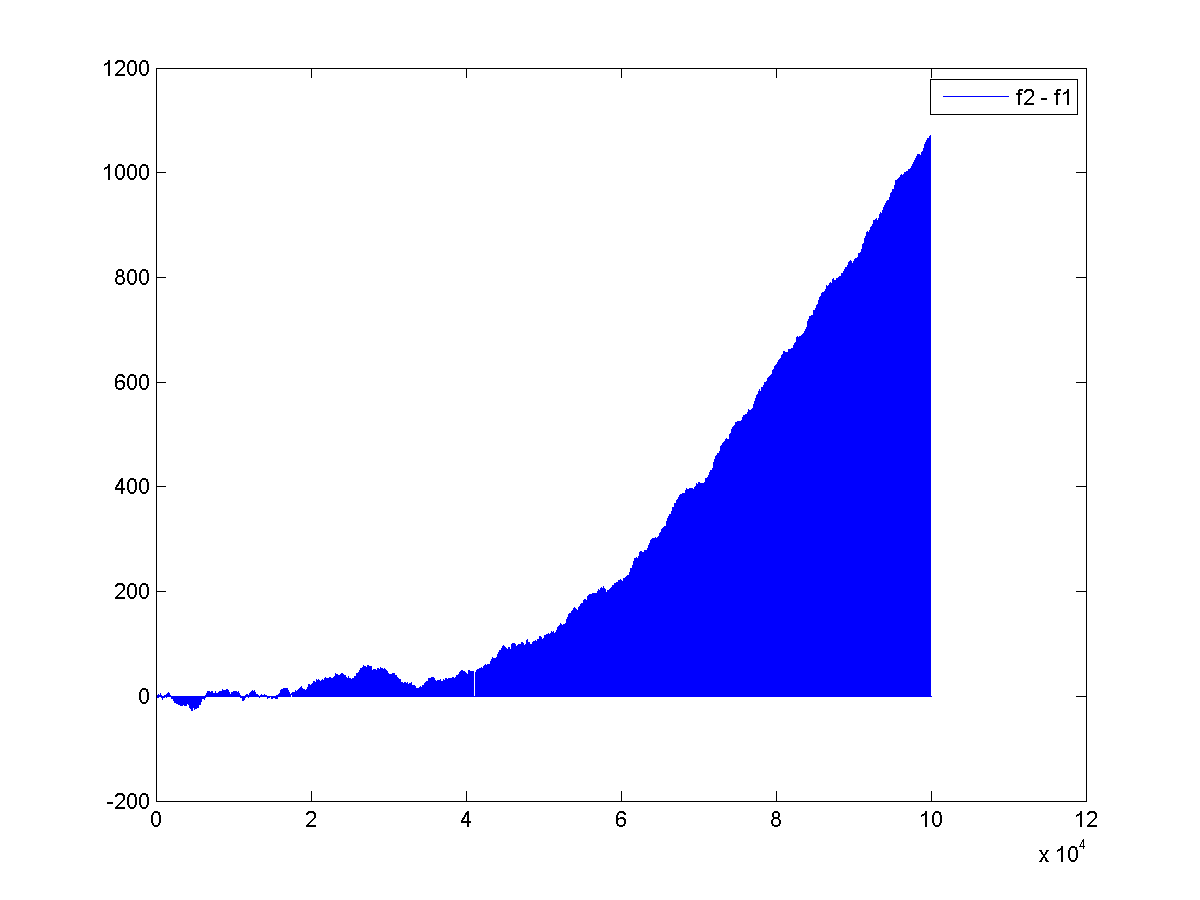
\includegraphics[scale=0.33]{Figures/base1/diff2_1} 
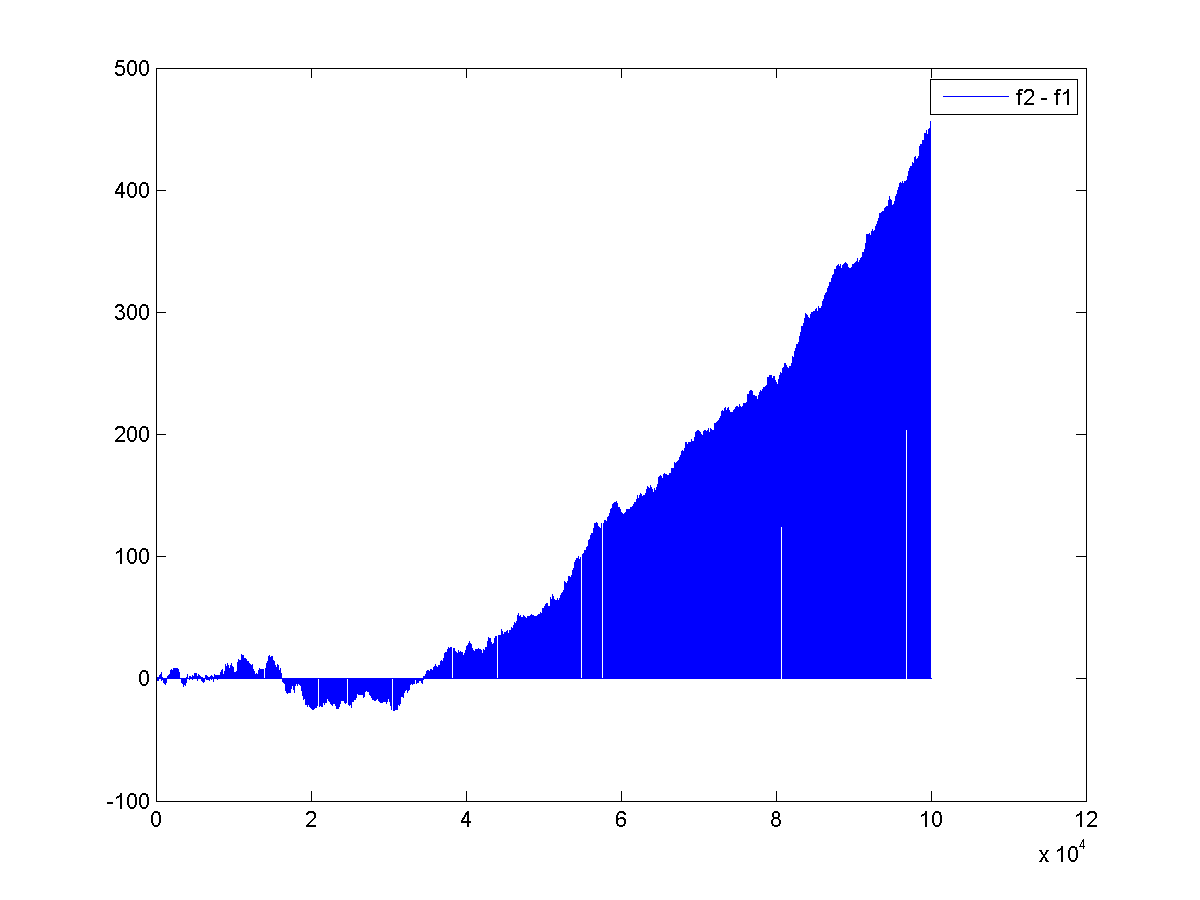
\includegraphics[scale=0.33]{Figures/base1/diff2_2} \\
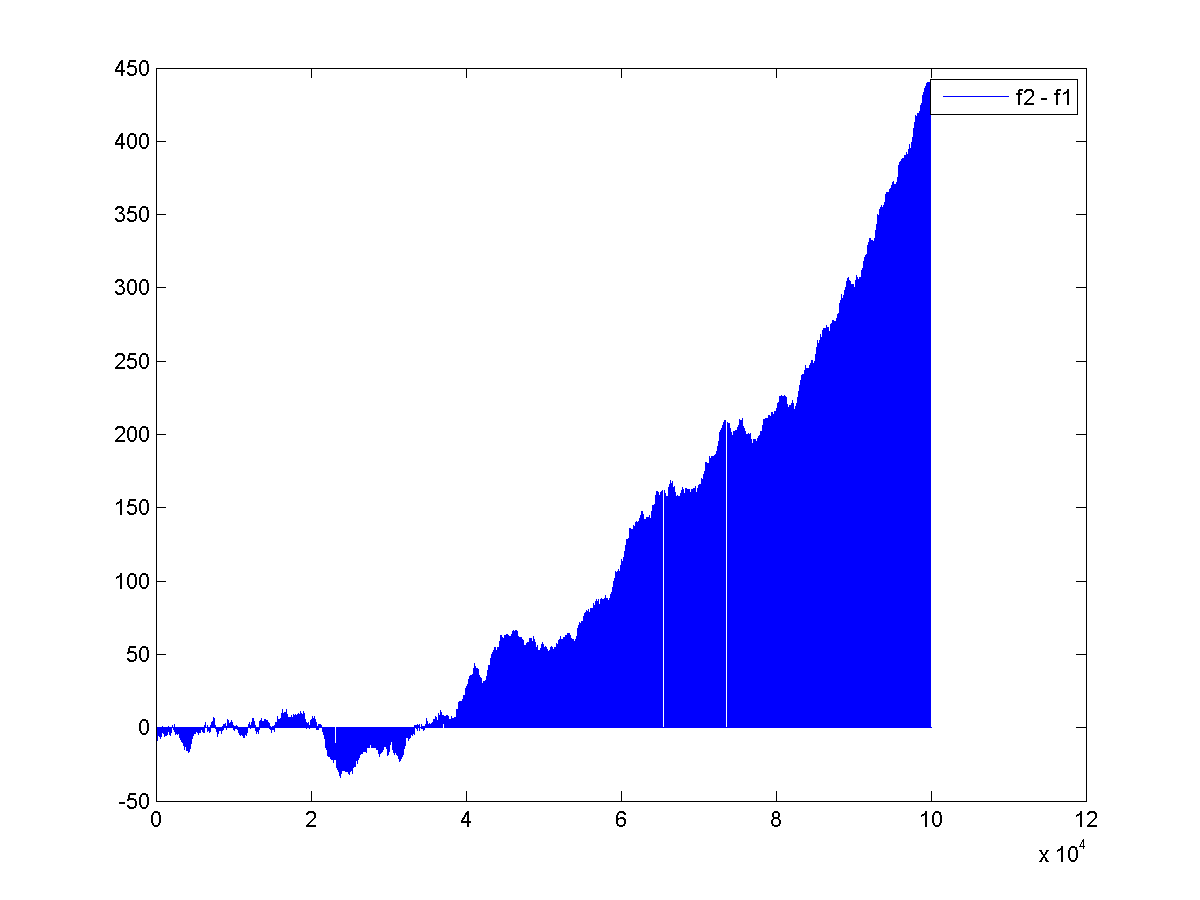
\includegraphics[scale=0.33]{Figures/base1/diff2_3}
\end{array}$
\end{center}
\caption{Difference 2}
\label{fig:diff2}
\end{figure}

\begin{figure}
\begin{center}$
\begin{array}{ccc}
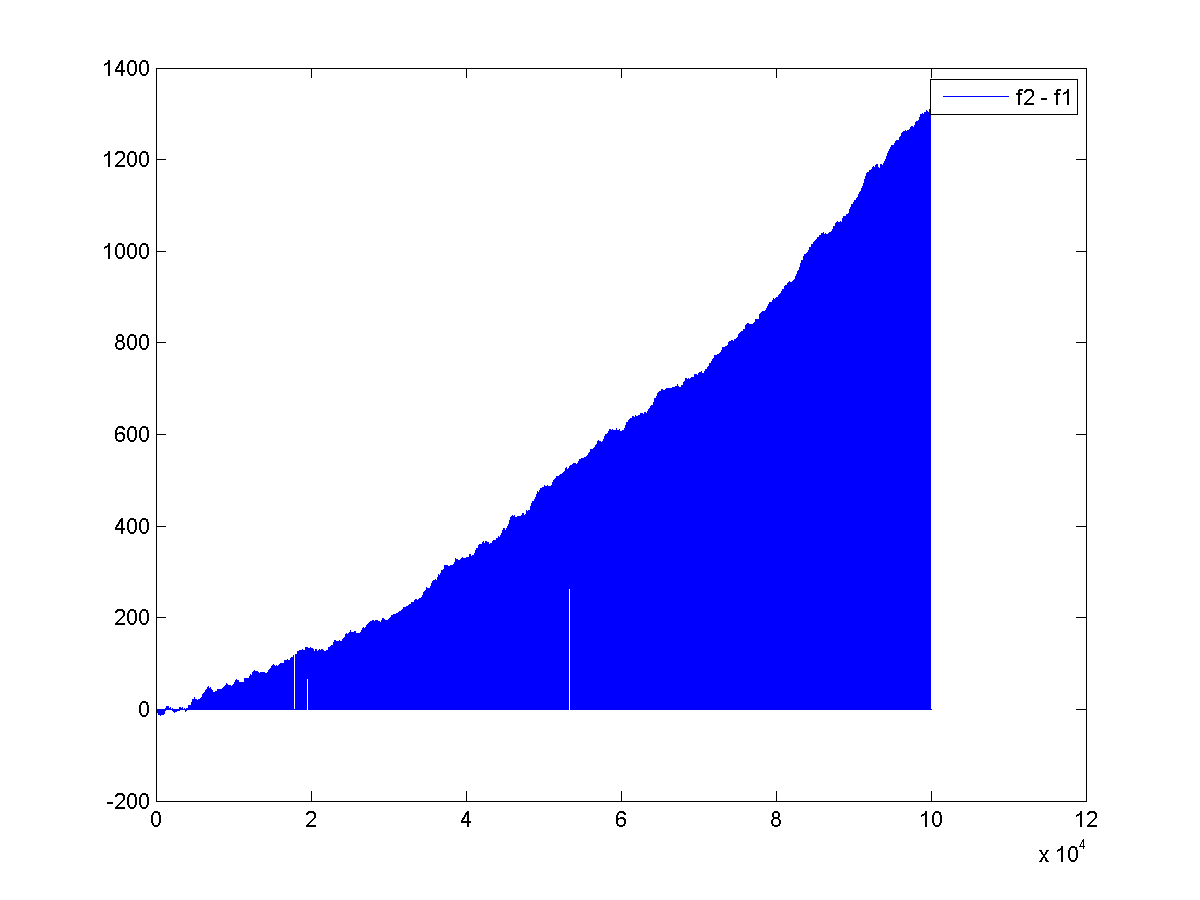
\includegraphics[scale=0.33]{Figures/base1/diff3_1} 
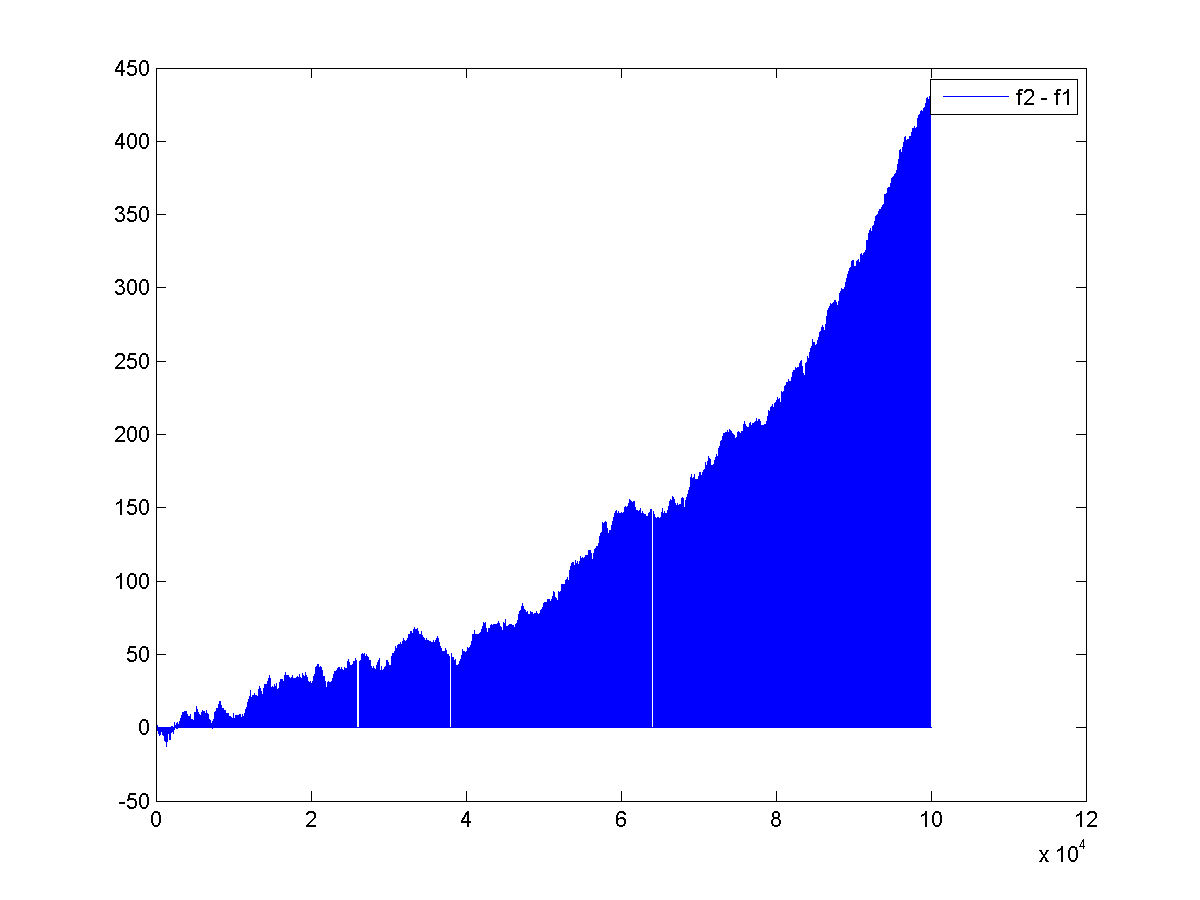
\includegraphics[scale=0.33]{Figures/base1/diff3_2} \\
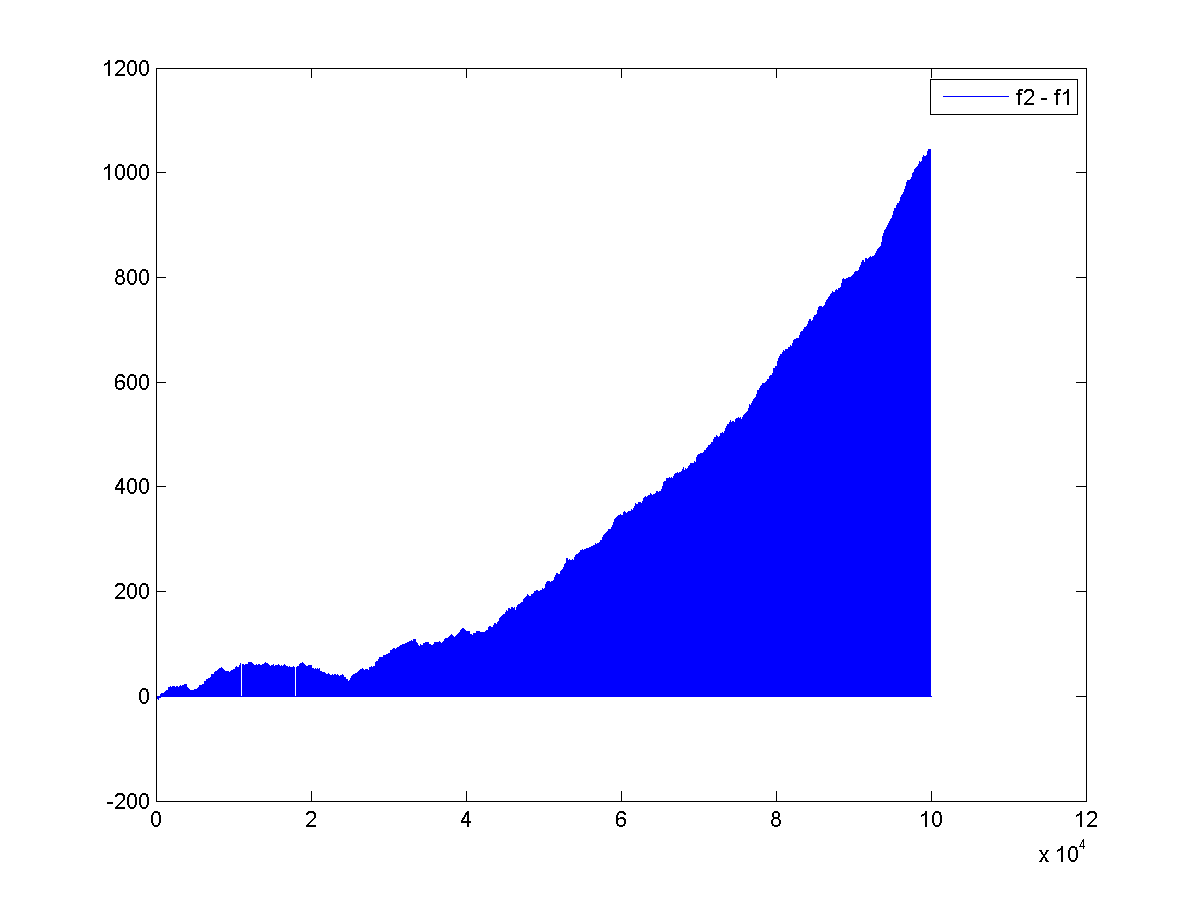
\includegraphics[scale=0.33]{Figures/base1/diff3_3}
\end{array}$
\end{center}
\caption{Difference 3}
\label{fig:diff3}
\end{figure}

\begin{figure}
\begin{center}$
\begin{array}{ccc}
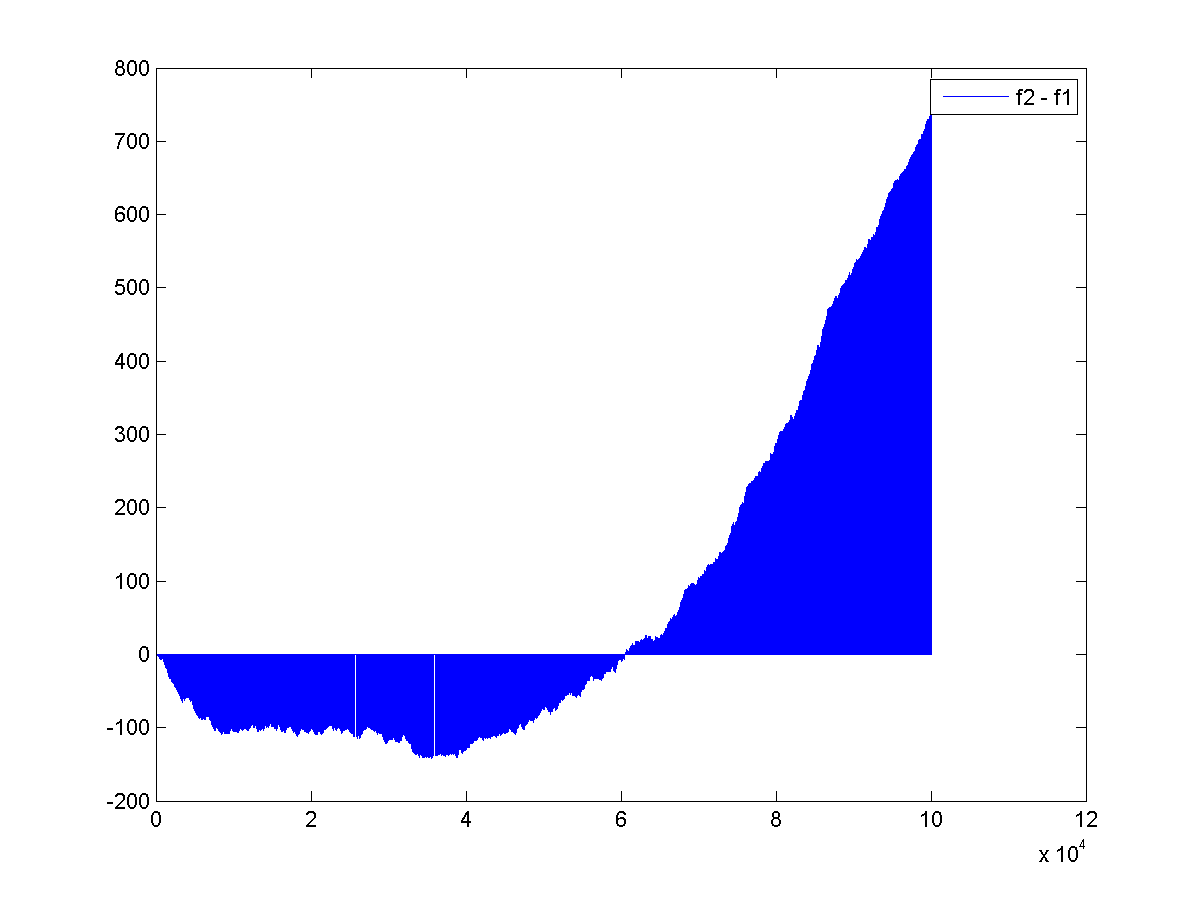
\includegraphics[scale=0.33]{Figures/base1/diff4_1} 
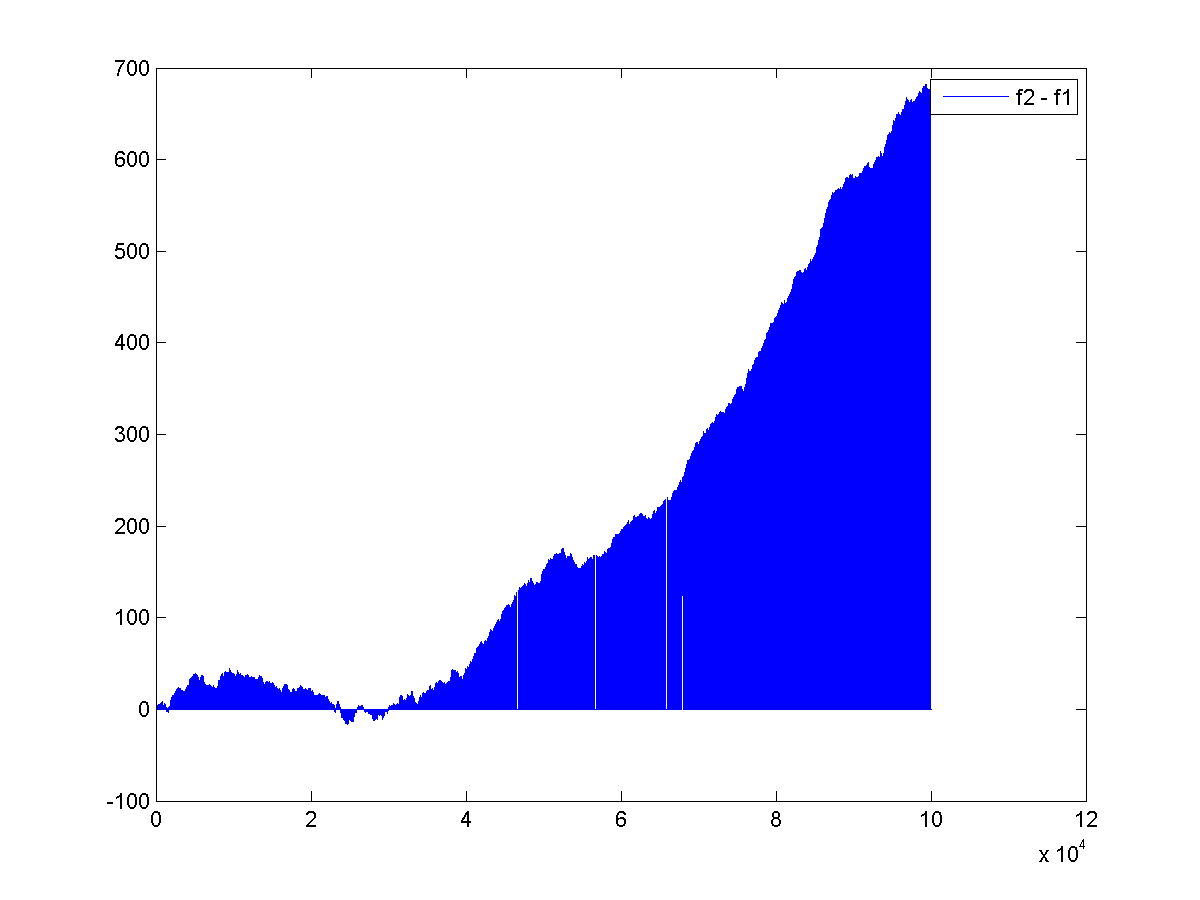
\includegraphics[scale=0.33]{Figures/base1/diff4_2} \\
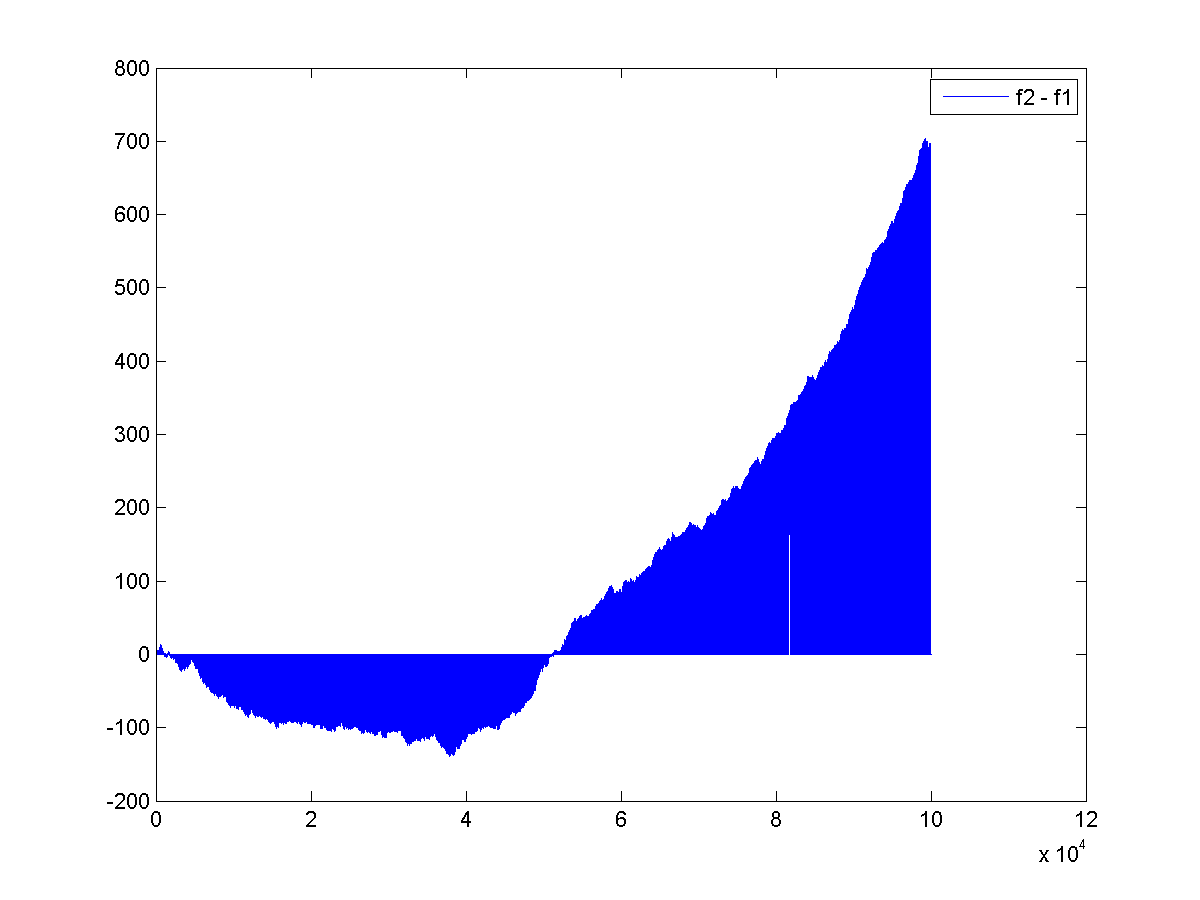
\includegraphics[scale=0.33]{Figures/base1/diff4_3}
\end{array}$
\end{center}
\caption{Difference 4}
\label{fig:diff4}
\end{figure}

\begin{figure}
\begin{center}$
\begin{array}{ccc}
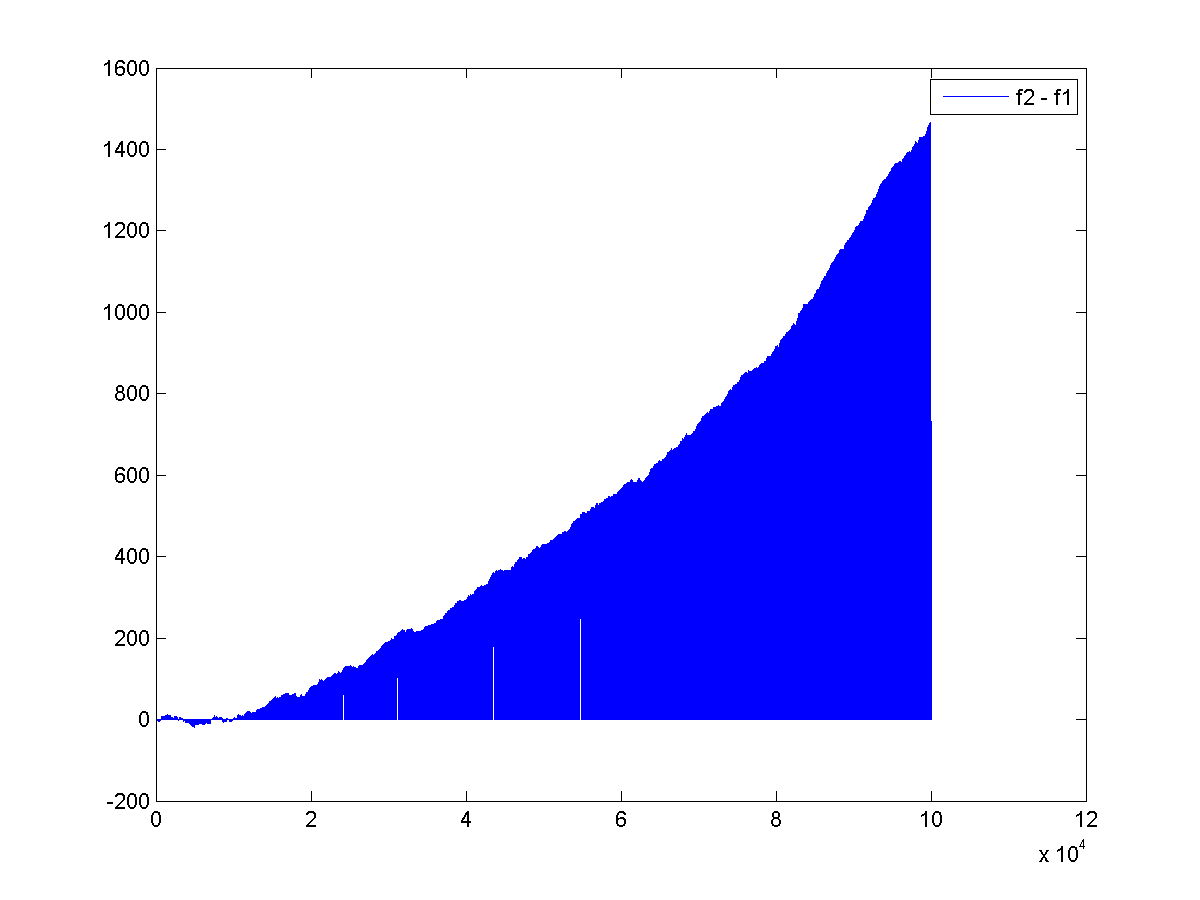
\includegraphics[scale=0.33]{Figures/base1/diff5_1} 
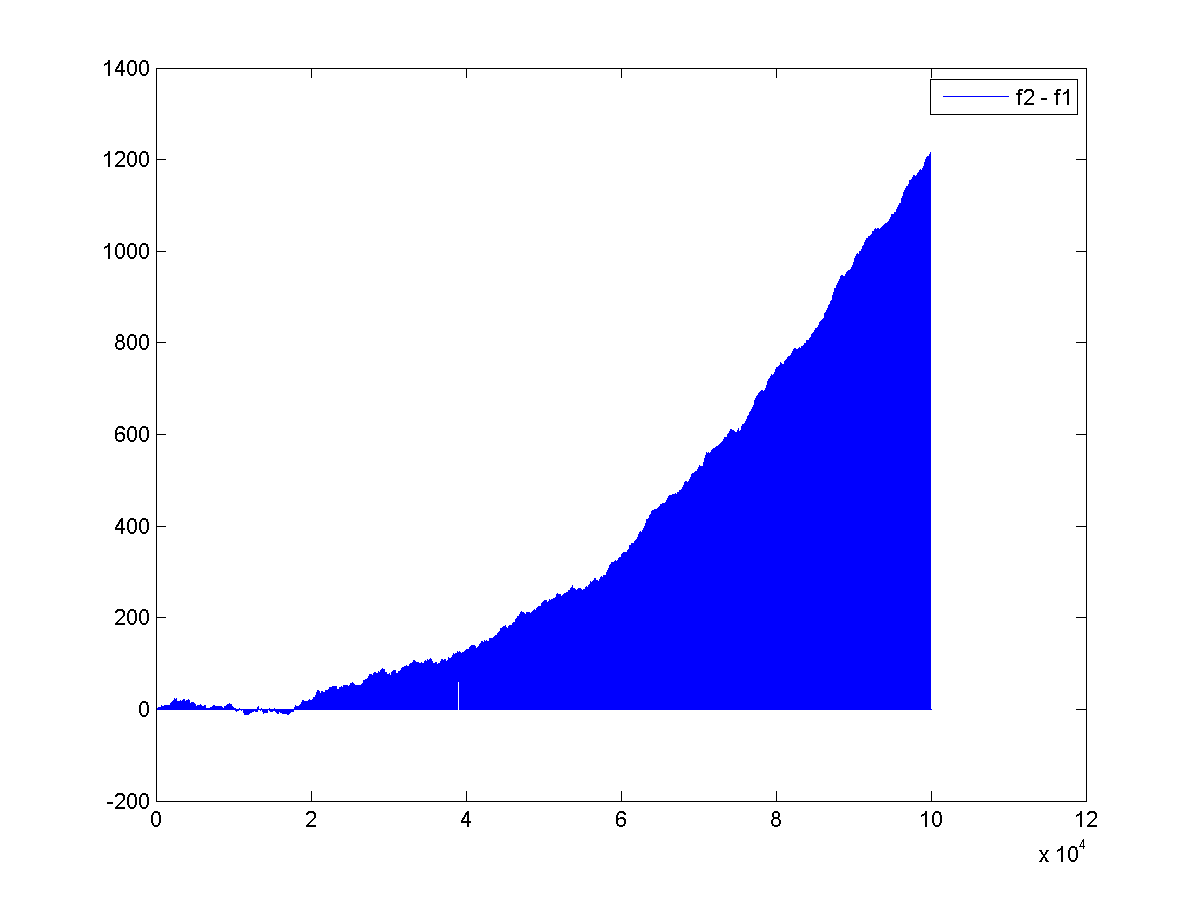
\includegraphics[scale=0.33]{Figures/base1/diff5_2} \\
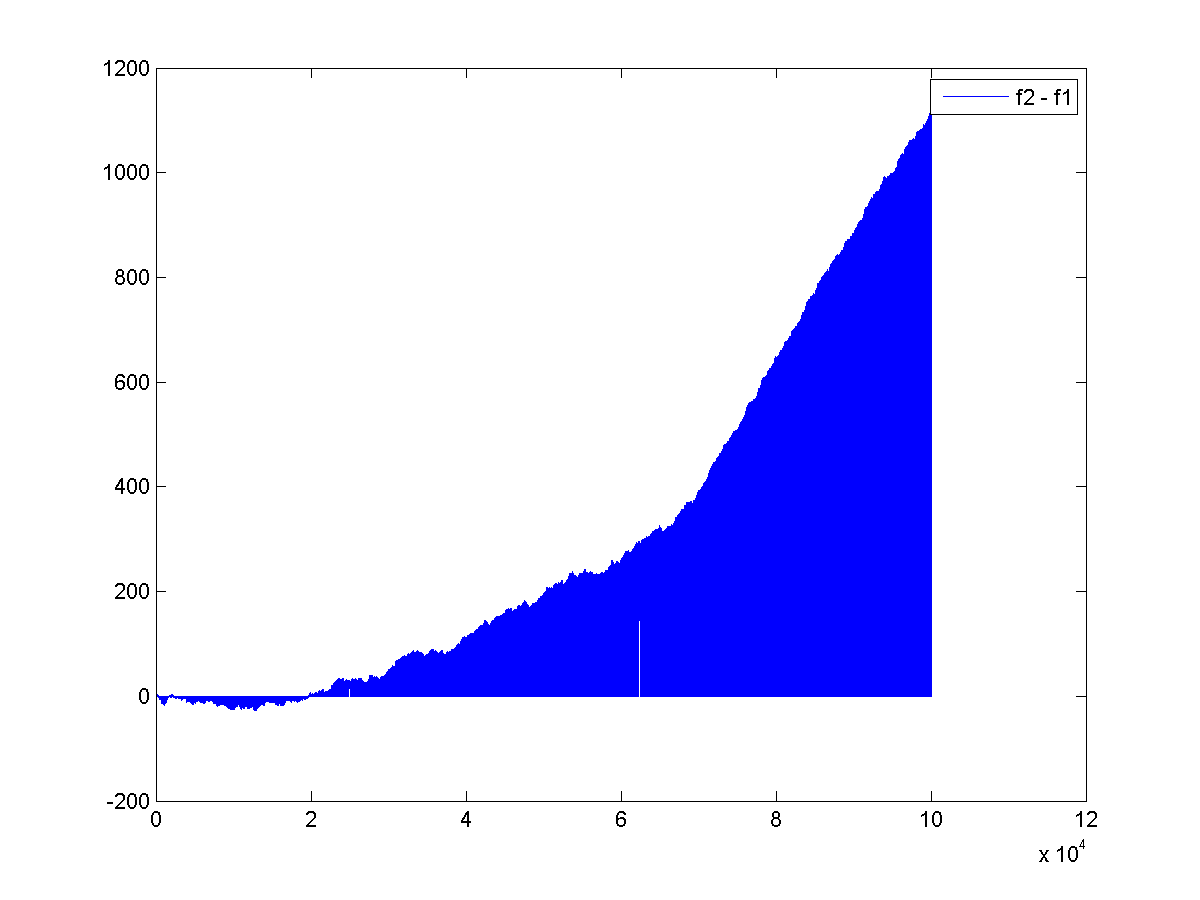
\includegraphics[scale=0.33]{Figures/base1/diff5_3}
\end{array}$
\end{center}
\caption{Difference 5}
\label{fig:diff5}
\end{figure}

\begin{figure}
\begin{center}$
\begin{array}{ccc}
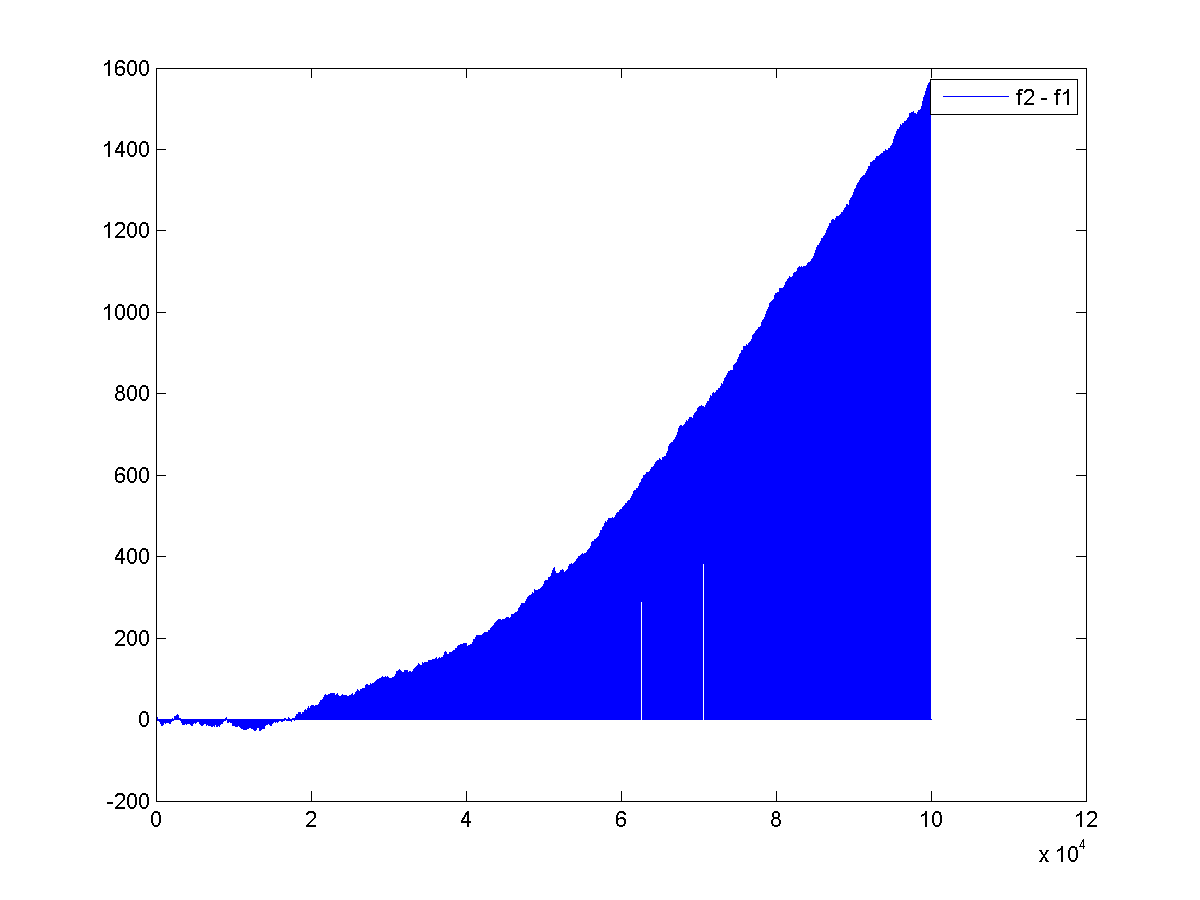
\includegraphics[scale=0.33]{Figures/base1/diff6_1} 
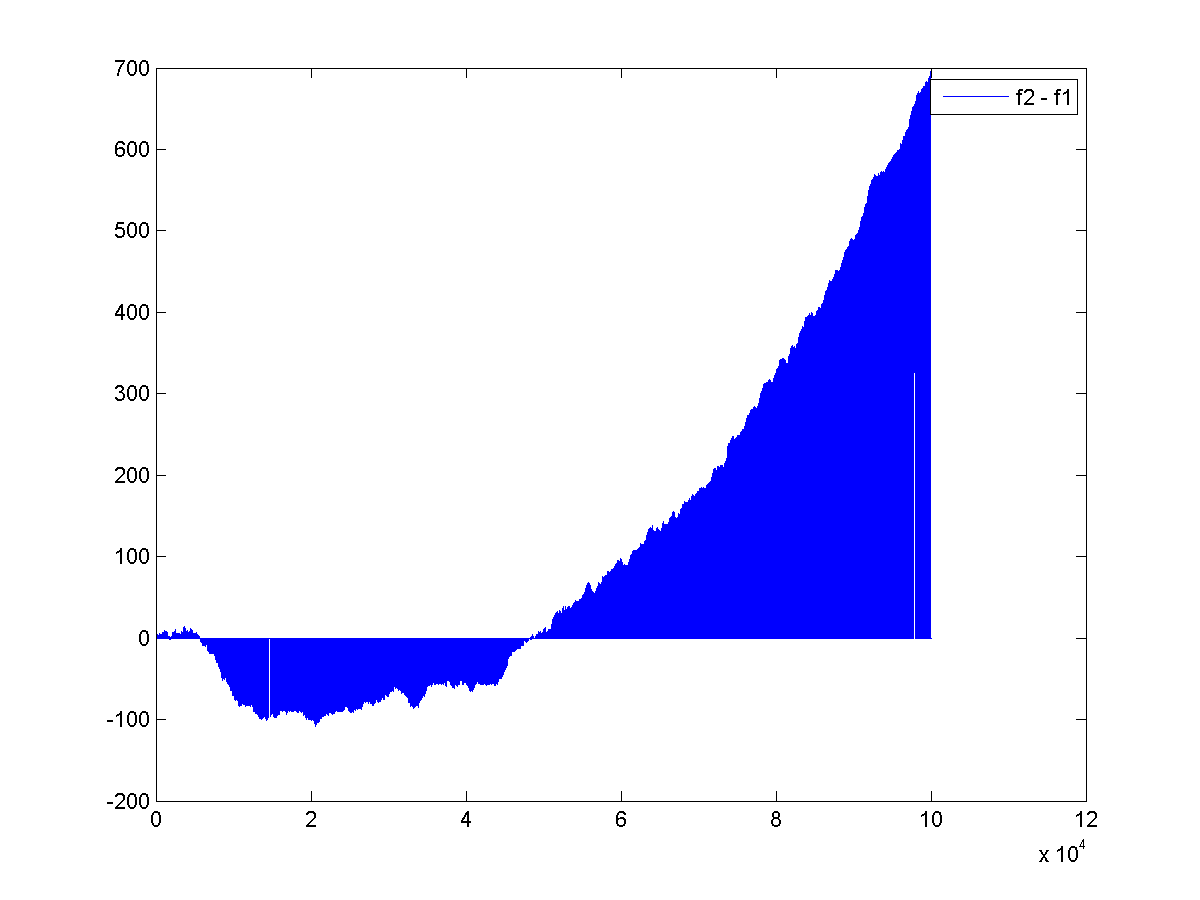
\includegraphics[scale=0.33]{Figures/base1/diff6_2} \\
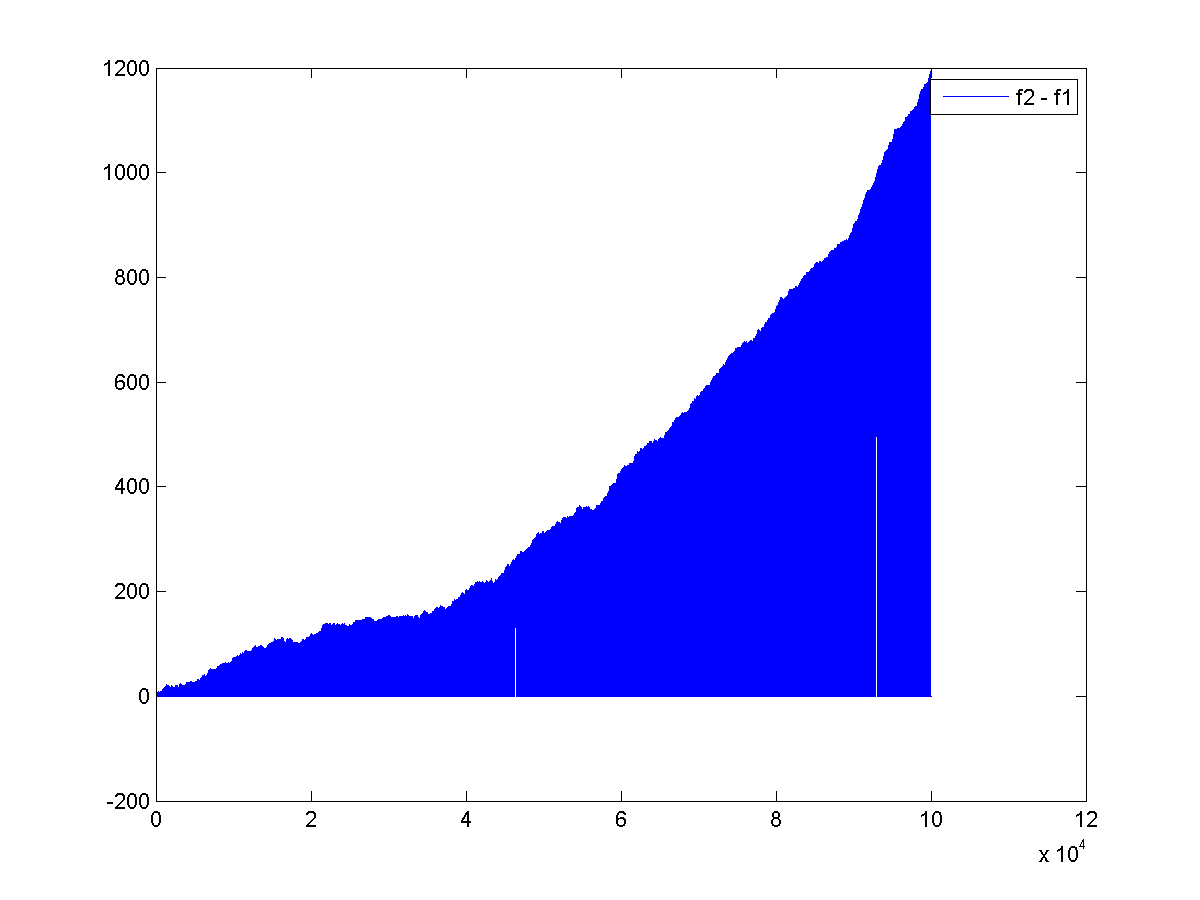
\includegraphics[scale=0.33]{Figures/base1/diff6_3}
\end{array}$
\end{center}
\caption{Difference 6}
\label{fig:diff6}
\end{figure}